% Copyright (c) Acconeer AB, 2026
% All rights reserved
\documentclass[tikz]{standalone}
\usepackage[utf8]{inputenc}
\usepackage[T1]{fontenc}
\usepackage{cmap}
\usepackage{amsmath}
\usepackage{amssymb}
\usepackage{verbatim}
\usepackage{bm}
\usepackage{siunitx}
\renewcommand{\familydefault}{\sfdefault}
\usepackage[cm]{sfmath}
\usepackage{tikz}
\usetikzlibrary{math}
\usetikzlibrary{bending}
\usetikzlibrary{decorations.pathreplacing}
\usetikzlibrary{decorations.pathmorphing}
\usetikzlibrary{fadings}
\usetikzlibrary{positioning}
\definecolor{cblue}{rgb}{0.396, 0.643, 0.82}
\definecolor{corange}{rgb}{1.0, 0.69, 0.416}
\definecolor{cgreen}{rgb}{0.471, 0.824, 0.471}
\definecolor{cred}{rgb}{1.0, 0.502, 0.502}
\definecolor{cpurple}{rgb}{0.863, 0.78, 0.937}
\def\symbsweeprate{f_s}
\def\symbsweepperiod{T_s}
\def\symbframerate{f_f}
\def\symbframeperiod{T_f}
\def\symbspf{N_s}
\def\symbnumpoints{N_d}
\def\symbnumchannels{N_c}
\begin{document}
% A121-style 2-D sweep/frame figure extended for the A212 by stacking N_c
% copies of the measurement matrix along a diagonal "channel" direction.
% The front slice carries all content (subsweeps, dots, labels, axes).
% Two lighter back-slices peek out at the upper-right to convey the stack.
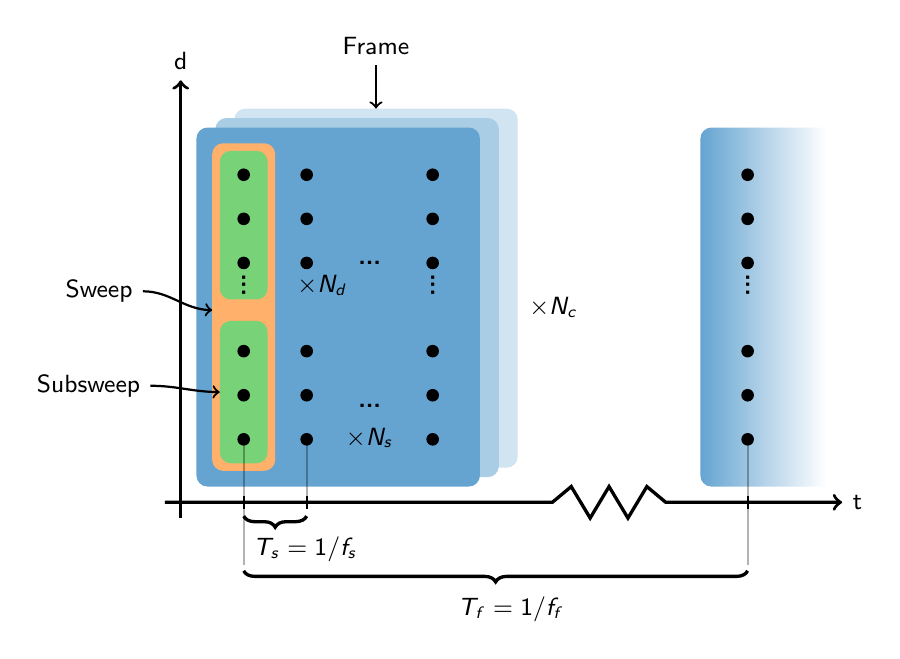
\begin{tikzpicture}[scale=0.8, font=\small]
  \tikzmath{
    \ph  = 0.7;
    \nump = 7;
    % Frame geometry (same as A121)
    \fw  = 4.5;
    \fh  = {(\nump-1)*\ph + 1.5};   % = 5.7
    \fxl = 0.25;
    \fyb = 0.25;
    % Sweep column geometry
    \sw  = 1.0;
    \sxl = 0.5;
    \syb = 0.5;
    % Sweep total height
    \sh  = {(\nump-1)*\ph + 1.0};    % = 5.2
    % Subsweep geometry: two green sub-bands within the orange sweep bar
    \ssha = 2.5;                      % lower subsweep height
    \sgap = 0.1;                      % gap between the two subsweeps
    \sshb = 2.6;                      % upper subsweep height
    \ssayb = \syb;                    % y-bottom of lower subsweep = 0.5
    \ssbyb = {\syb + \ssha + \sgap};  % y-bottom of upper subsweep = 2.3
    % Insets so orange is visible around each green bar
    \gpadx = 0.12;   % horizontal inset on each side
    \gpady = 0.12;   % vertical inset on top and bottom of each bar
    % Channel-stack: each back-slice is offset by (sdx, sdy)
    \sdx = 0.3;
    \sdy = 0.15;
  }
  % ===== CHANNEL STACK: back slices (drawn first, lightest at back) =====
  % Slice 3 (back-most)
  \fill [fill=cblue!30, rounded corners]
    ({\fxl+2*\sdx}, {\fyb+2*\sdy}) rectangle ++(\fw, \fh);
  % Slice 2
  \fill [fill=cblue!55, rounded corners]
    ({\fxl+\sdx}, {\fyb+\sdy}) rectangle ++(\fw, \fh);
  % ===== FRONT SLICE (Slice 1, fully drawn) =====
  \fill [fill=cblue, rounded corners] (\fxl, \fyb) rectangle ++(\fw, \fh);
  % Fading "next frame" stub (front slice only)
  \fill [fill=cblue, rounded corners, path fading=east]
    (10.25, \fyb) -- ++(-2, 0) -- ++(0, \fh) -- ++(2, 0);
  % ===== SWEEP AND SUBSWEEP BOXES (on the front slice) =====
  % Full orange sweep bar (the overall sweep envelope)
  \fill [fill=corange, rounded corners] (\sxl, \syb) rectangle ++(\sw, \sh);
  % Green subsweep bars --inset so orange is visible on all four sides
  \fill [fill=cgreen, rounded corners]
    ({\sxl+\gpadx}, {\ssayb+\gpady}) rectangle ++({\sw-2*\gpadx}, {\ssha-2*\gpady});
  \fill [fill=cgreen, rounded corners]
    ({\sxl+\gpadx}, {\ssbyb+\gpady}) rectangle ++({\sw-2*\gpadx}, {\sshb-2*\gpady});
  % ===== LABELS =====
  % "Subsweep" -- arrowhead on green bar's left edge, label to the left of figure
  \draw [<-, thick] ({\sxl+\gpadx}, {\ssayb+\gpady+(\ssha-2*\gpady)*0.5})
    to [out=180, in=0] ++(-1.1, 0.1) node [left] {Subsweep};
  % "Sweep" -- arrowhead on orange left edge in the gap between the two subsweeps
  \draw [<-, thick] (\sxl, {\ssayb + \ssha + \sgap * 0.5})
    to [out=180, in=0] ++(-1.1, 0.3) node [left] {Sweep};
  % "Frame" -- arrow from top-centre of stack, pointing upward to label
  \draw [<-, thick] ({\fxl+2*\sdx+\fw*0.5}, {\fyb+2*\sdy+\fh})
    to ++(0, 0.7) node [above] {Frame};
  % ===== CHANNEL-DEPTH ANNOTATION =====
  % Label to the right of the stack at mid-frame height
  \node [right, inner sep=4pt]
    at ({\fxl+\fw+2*\sdx}, {\fyb+\fh*0.5})
    {$\times \symbnumchannels$};
  % ===== MEASUREMENT POINTS =====
  % Rows i=1,2,3 fall in SS-a (unshifted x-columns).
  \foreach \i in {1, 2, 3} {
    \tikzmath{ \yy = (\i-1)*\ph; }
    \foreach \x in {0, 1, 3, 8.0} {
      \fill [fill=black] (\x + 1, \yy + 1) circle (1mm);
    }
  }
  % Rows i=5,6,7 fall in SS-b.
  \foreach \i in {5, 6, 7} {
    \tikzmath{ \yy = (\i-1)*\ph; }
    \foreach \x in {0, 1, 3, 8.0} {
      \fill [fill=black] (\x + 1, \yy + 1) circle (1mm);
    }
  }
  % "..." for more distance points (shown between the last two dot rows)
  \foreach \x in {0, 3, 8.0} {
    \node[rotate=90] at (\x + 1, {3.5*\ph+1}) {$\bm\ldots$};
  }
  \node at (2.25, {3.5*\ph+1}) {$\times \symbnumpoints$};
  % "..." for more sweeps within the frame
  \node at (3, {0.5*(2.5-1)*\ph+1})   {$\bm\ldots$};
  \node at (3, {4*\ph+1})              {$\bm\ldots$};
  \node at (3, {0.5*(2.5-1)*\ph+0.5}) {$\times \symbspf$};
  % ===== AXES =====
  % t-axis (time) -- single axis-break tooth centred in the inter-frame gap (x~6.8)
  \draw [->, very thick] (-0.25, 0) -- (5.9, 0)
    -- (6.2, 0.25) -- (6.5, -0.25) -- (6.8, 0.25) -- (7.1, -0.25) -- (7.4, 0.25) -- (7.7, 0) -- (10.5, 0) node[right]{t};
  % d-axis (distance)
  \draw [->, very thick] (0, -0.25) -- (0, {(\nump-1)*\ph+2.5}) node[above]{d};
  % ===== TIMING ANNOTATIONS =====
  % Tick marks on t-axis
  \foreach \x in {1, 2, 9.0} {
    \draw [thick] (\x, 0.1) -- ++(0, -0.2);
  }
  % Faint vertical reference lines
  \draw [thick, opacity=0.3] (1, 1) -- (1, -1);
  \draw [thick, opacity=0.3] (9.0, 1) -- ++(0, -2);
  \draw [thick, opacity=0.3] (2, 1) -- (2, 0);
  % Sweep period brace
  \draw [very thick, decoration={brace, amplitude=4pt, mirror, raise=5pt}, decorate]
    (1, 0) -- (2, 0);
  \node [right] at (1, -0.75) {$\symbsweepperiod = 1/\symbsweeprate$};
  % Frame period brace
  \draw [very thick, decoration={brace, amplitude=4pt, mirror, raise=2pt}, decorate]
    (1, -1.0) -- (9.0, -1.0);
  \node [right] at (4.25, -1.7) {$\symbframeperiod = 1/\symbframerate$};
\end{tikzpicture}
\end{document}
